\documentclass[../main]{subfiles}
\newcommand*\circled[1]{\tikz[baseline=(char.base)]{
            \node[shape=circle,draw,inner sep=1pt] (char) {#1};}}
    \begin{document}
    \setcounter{secnumdepth}{2}
    \chapter{提案手法}
        \section{全天球カメラに基づく通路認識手法}
        本研究は,全天球カメラから取得した画像に基づき,通路認識を行う手法の検証を行う.ここでいう通路認識とは,画像中に通路があるかどうかを検出するだけでなく,
        画像中に通路がある場合,その通路がどのタイプに属するのかといった,通路の特徴(形状)情報を取得することである.また,本研究で扱う通路のタイプは以下の
        8種類であり,図を\fref{figure::new_aisle_type}に示す.\\
         \circled{1}一本道(straight)\\
         \circled{2}行き止まり(dead end)\\
         \circled{3}右のみ曲がれる角(right)\\
         \circled{4}左のみ曲がれる角(left)\\
         \circled{5}十字路(cross)\\
         \circled{6}右に曲がれる三叉路(3-way junction\_right)\\
         \circled{7}左に曲がれる三叉路(3-way junction\_left)\\
         \circled{8}突き当たりの三叉路(3-way junction\_center)
       
        %8タイプの通路の画像例
        \begin{figure}[H]
            \centering
            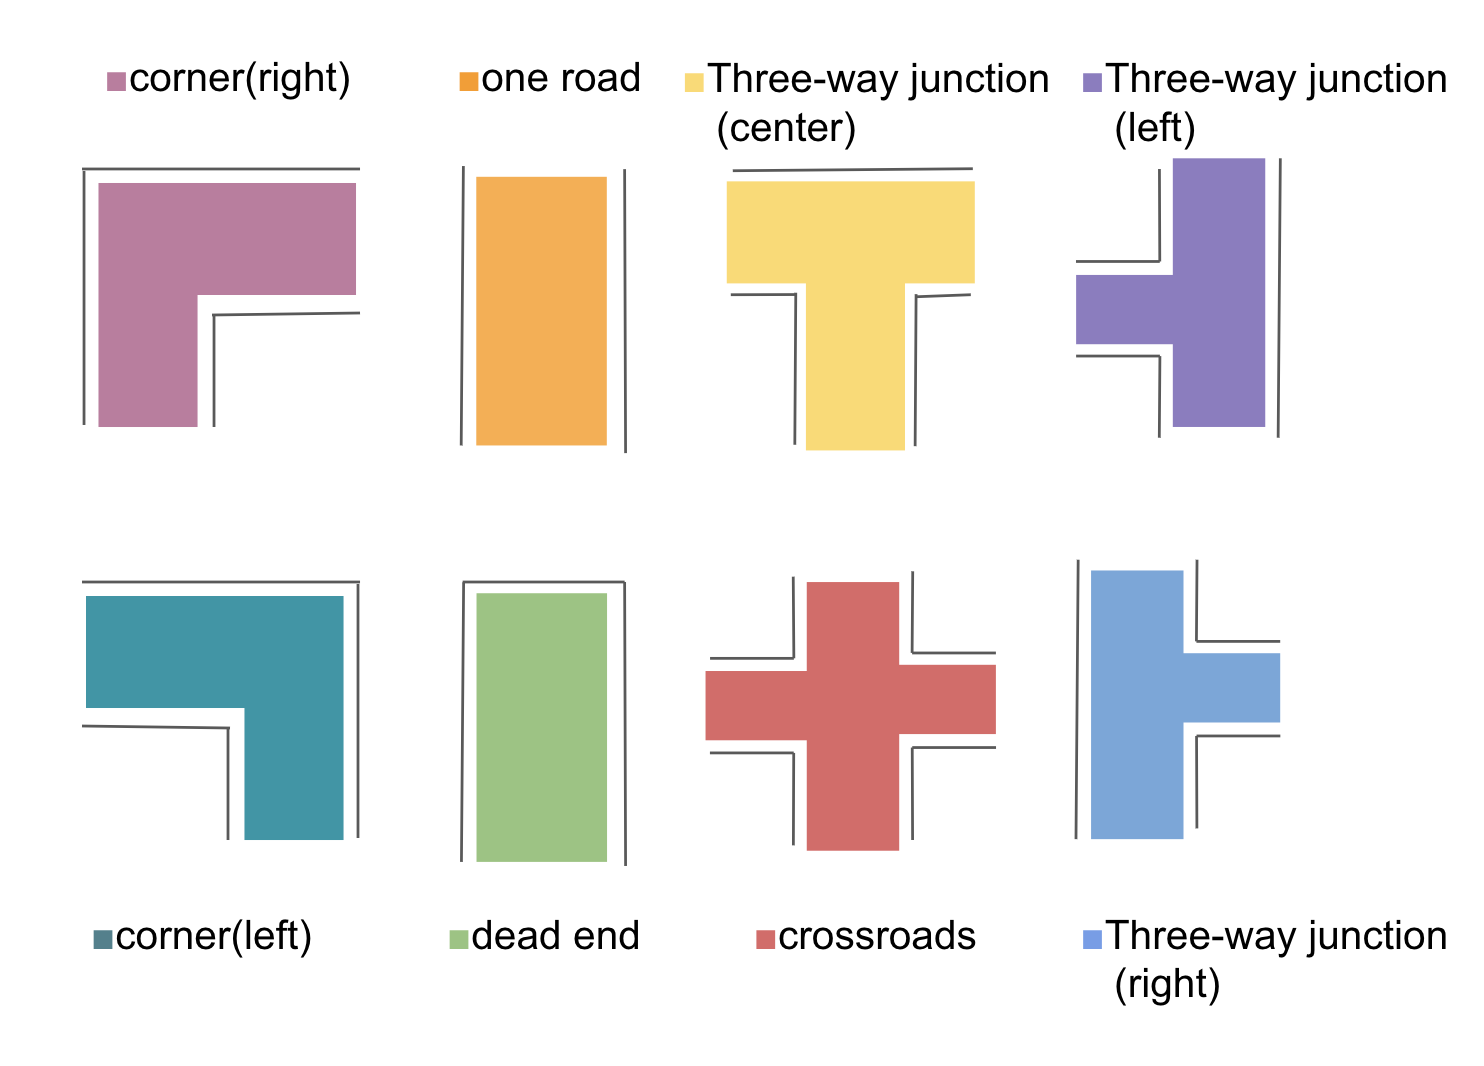
\includegraphics[width=10cm]{../images/new_aisle_type.png}
            \caption{Type of passage.}
            \label{figure::new_aisle_type}
        \end{figure}
        
        \newpage

        本手法の通路認識の流れを\fref{figure::proposed_method_fig}に示す.
        まず,全天球カメラ画像のRGBデータをYOLOの入力とし,出力された情報をもとに画像中に通路があるかどうかを検出する.
        画像中に通路が検出された場合,バウンディングボックスにより得られる画像中の通路の座標に基づき,通路のタイプを決定する.
        
        %提案手法の簡単な例
        \begin{figure}[H]
            \centering
            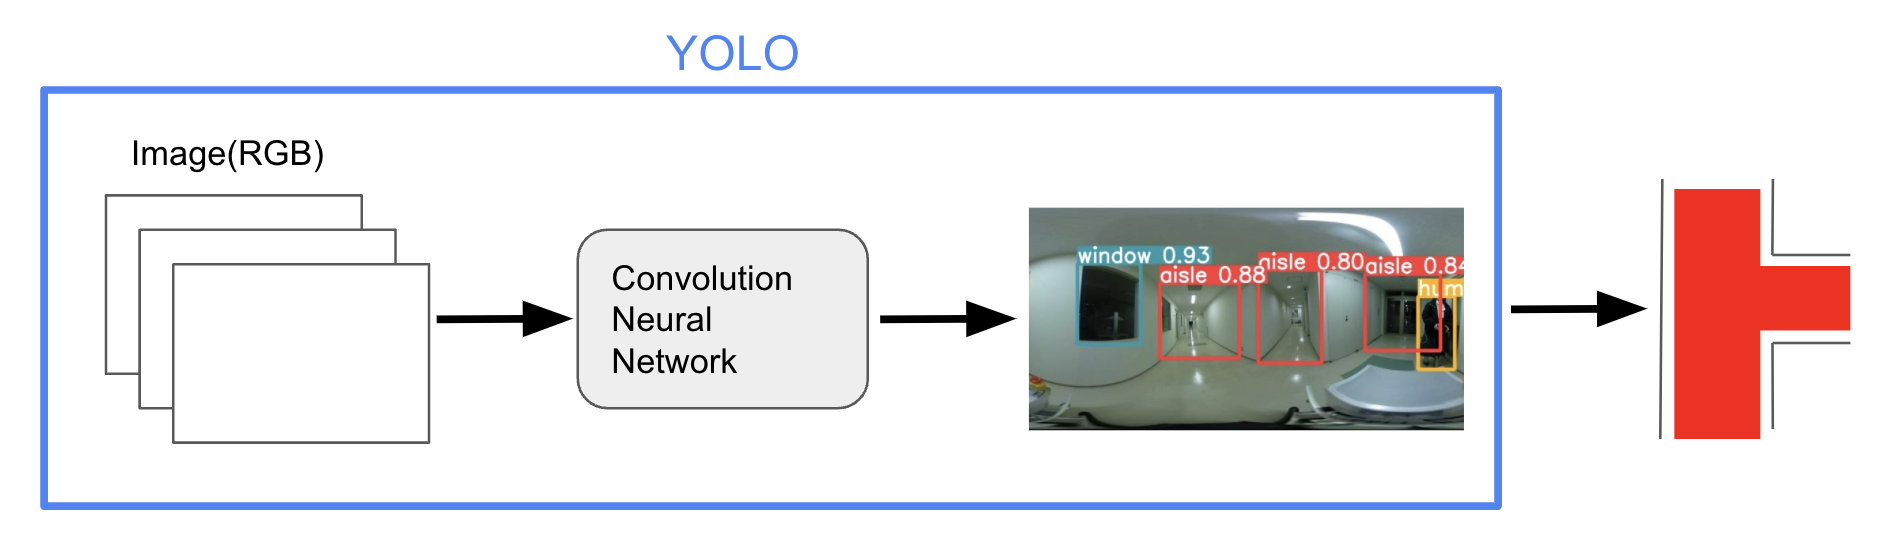
\includegraphics[width=10cm]{../images/proposed_method2.png}
            \caption{Flow of passage recognition method.}
            \label{figure::proposed_method_fig}
            この例では,画像から通路が3つ検出されている.また,通路はロボットに対して\\
            前方,後方,右手側に検出されているため,タイプは三叉路であるということがわかる.
        \end{figure}

        \newpage
        
        何も手を加えていない状態の全天球カメラ画像は,\fref{subfigure::no_proc}に示すように後方の通路が見切れてしまう.この状態の画像で学習を行なった結果,
        見切れた状態の通路が学習に影響を与え,通路認識に支障が出てしまった.
        そこで,\fref{subfigure::preproc}に示すような画像の前処理を行なった.この処理では,320*640の全天球カメラ画像の左端を切り取り,
        右端に貼り付けるということを行なった.

        YOLOのモデル作成のため,自作のデータセットにより学習を行う.学習に使うデータは津田沼キャンパス2号館3階で収集した.
        また,データセットの一例を\fref{figure::dataset_fig}に示す.また,データセットのクラスは\tref{table::datasets_table}の11クラスで設定した.
        先行研究では,8つの形状タイプの通路の認識を行なったため,本研究でも先行研究と同様の通路認識を行う.
        次に,YOLOの出力として得られた通路の情報に基づき,を参考にし,画像中の通路が認識された箇所を場合分けし,通路の形状を決定する.
        
        %画像の前処理の例
        \begin{figure}[htbp]
          \centering
           \subfigure[no processing image]{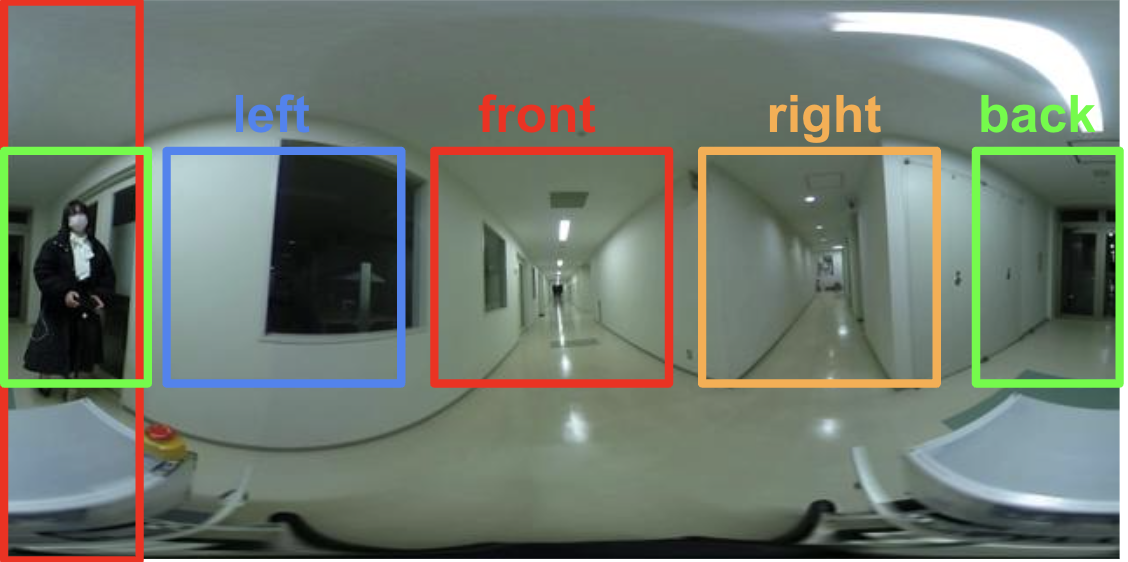
\includegraphics[height=4cm]{../images/no_processing.png}
           \label{subfigure::no_proc}}
           \subfigure[preprocessing image]{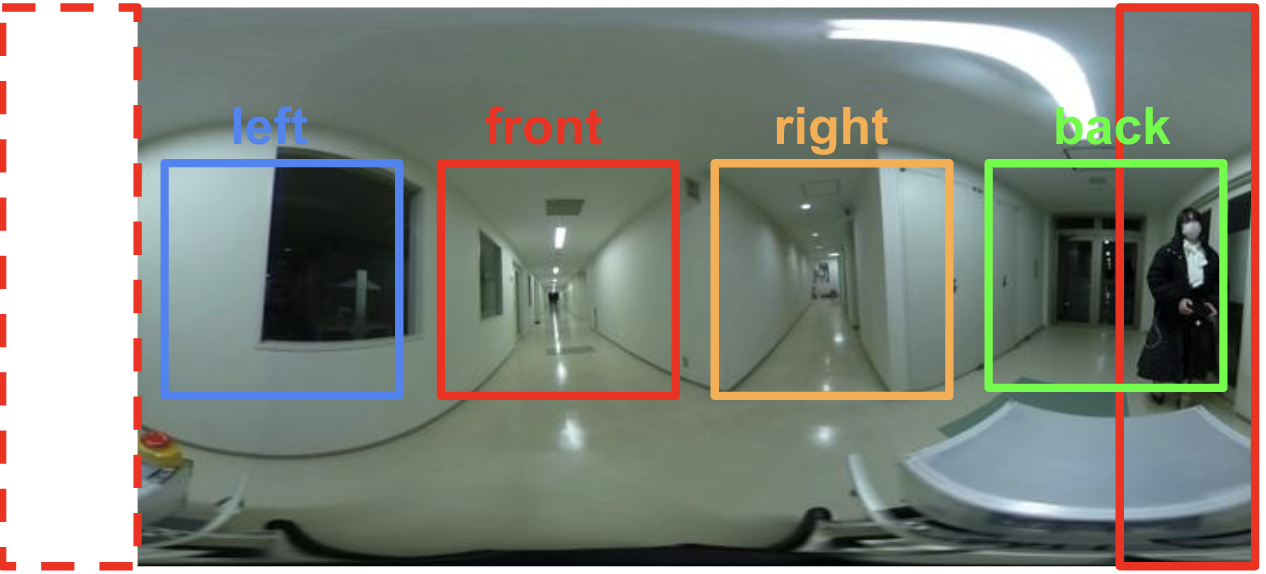
\includegraphics[height=4cm]{../images/after_processing.png}
           \label{subfigure::preproc}}
           \caption{Preprocessing of spherical camera images}
           \label{figure::proc_exp}
        \end{figure}

        %自作データセットの画像例
        \begin{figure}[H]
         \centering
         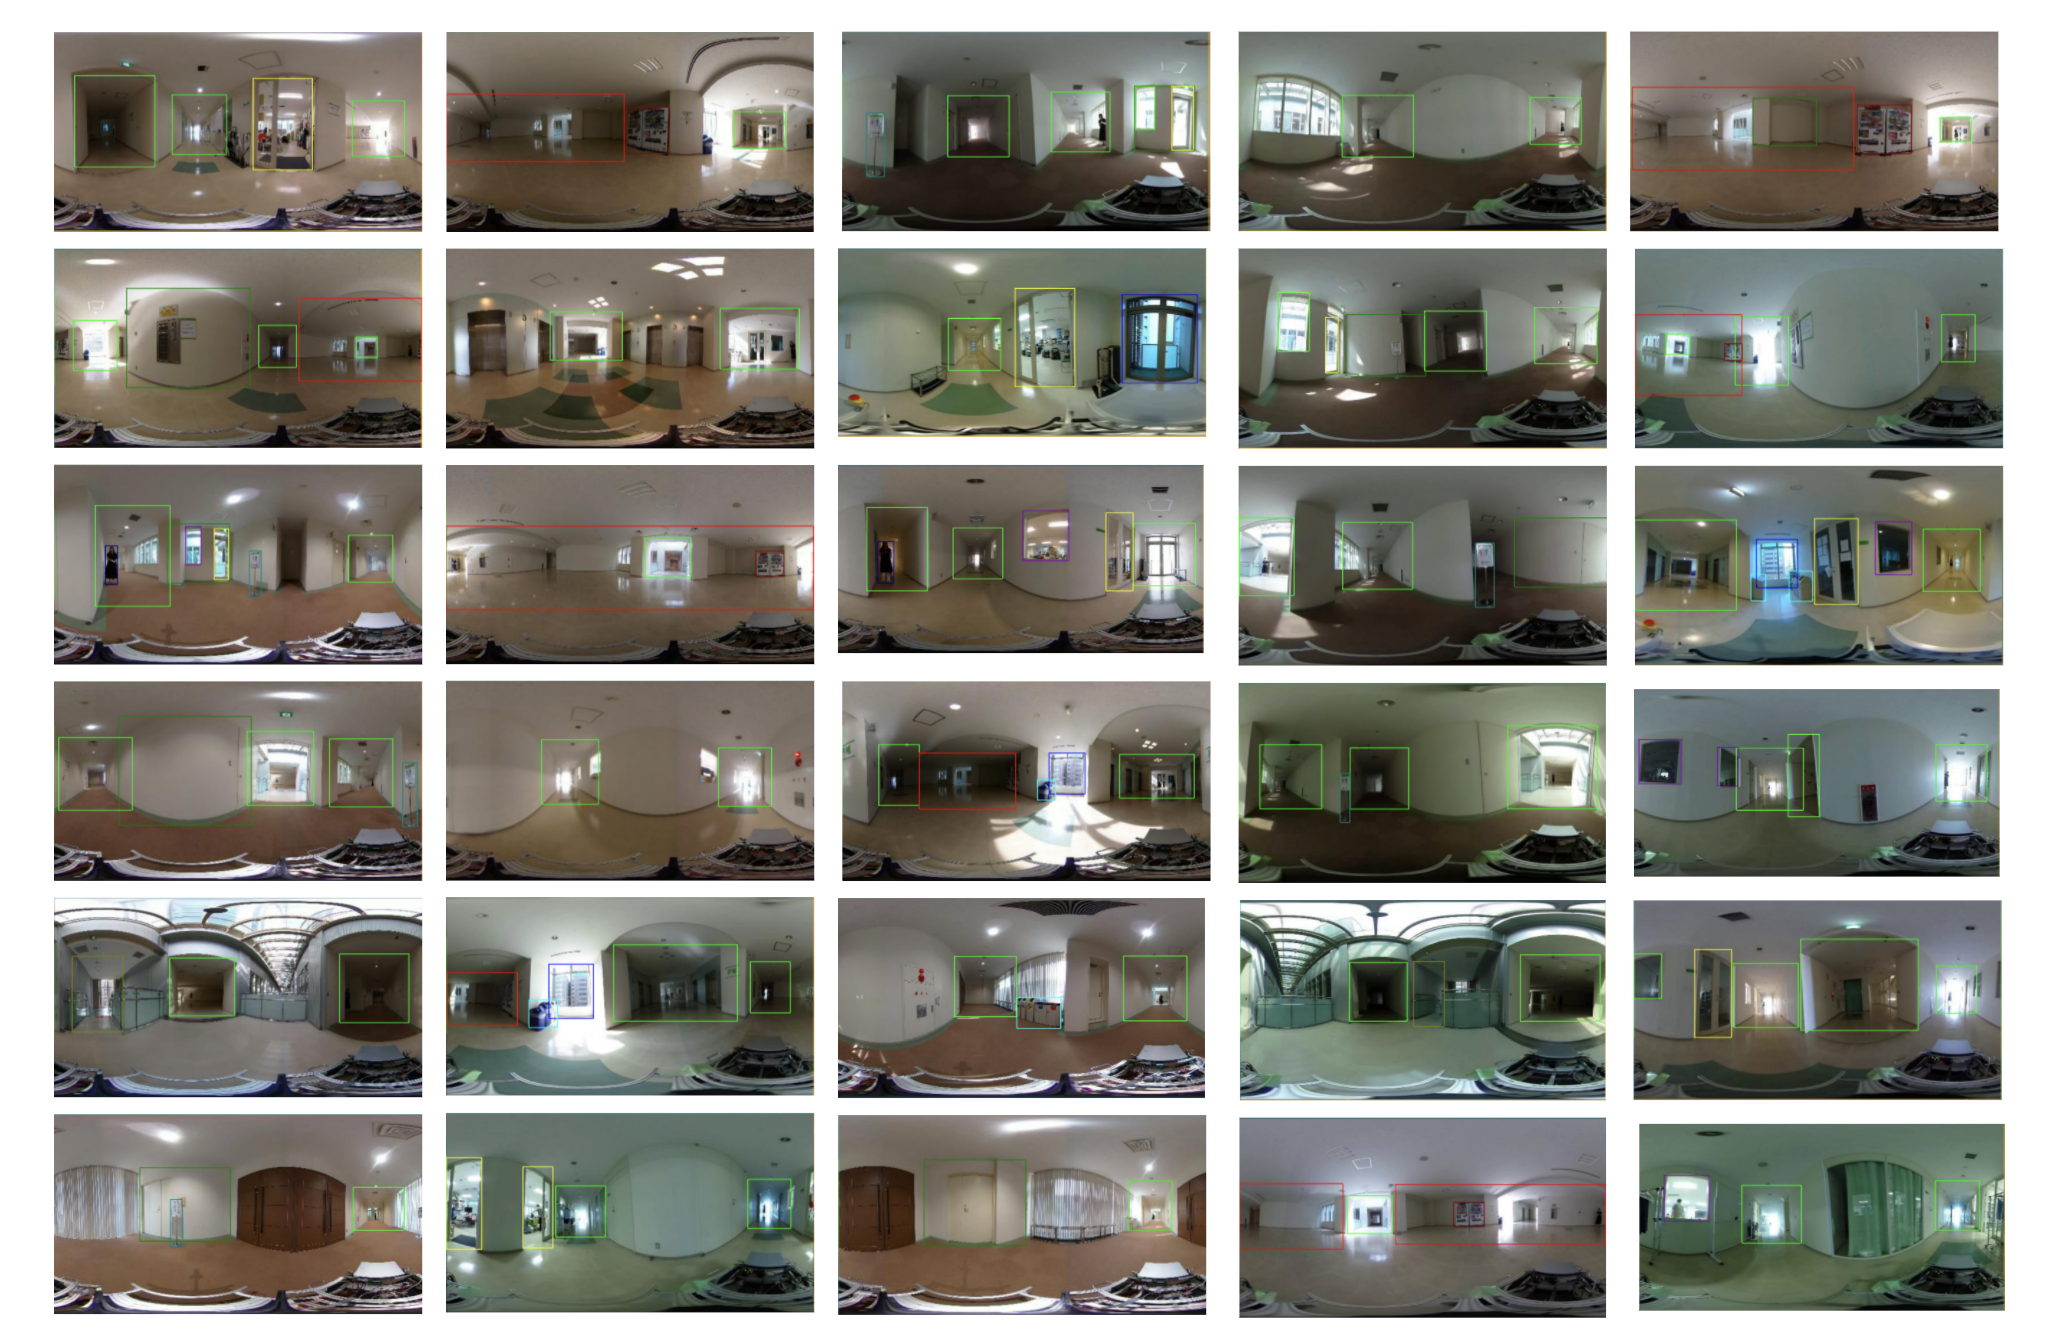
\includegraphics[width=10cm]{../images/dataset_exp.png}
         \caption{An example of a dataset.}
         \label{figure::dataset_fig}
        \end{figure}

        %データセットのクラス数
        \begin{table}[H]
            \caption{Class name to be labeled.}
            \centering
            \label{table::datasets_table}
            \begin{tabular}{lllll}
            \hline
            name of the class &  &  &  &  \\ 
            \hline \hline
            aisle             &  &  &  &  \\
            end               &  &  &  &  \\
            door\_end         &  &  &  &  \\
            human             &  &  &  &  \\
            door              &  &  &  &  \\
            step              &  &  &  &  \\
            square            &  &  &  &  \\
            vending\_machine  &  &  &  &  \\
            trash\_can        &  &  &  &  \\
            signboard         &  &  &  &  \\
            window            &  &  &  &  \\ 
            \hline
            \end{tabular}
        \end{table}
\end{document}

%\begin{figure}[H]
        %\centering  
        %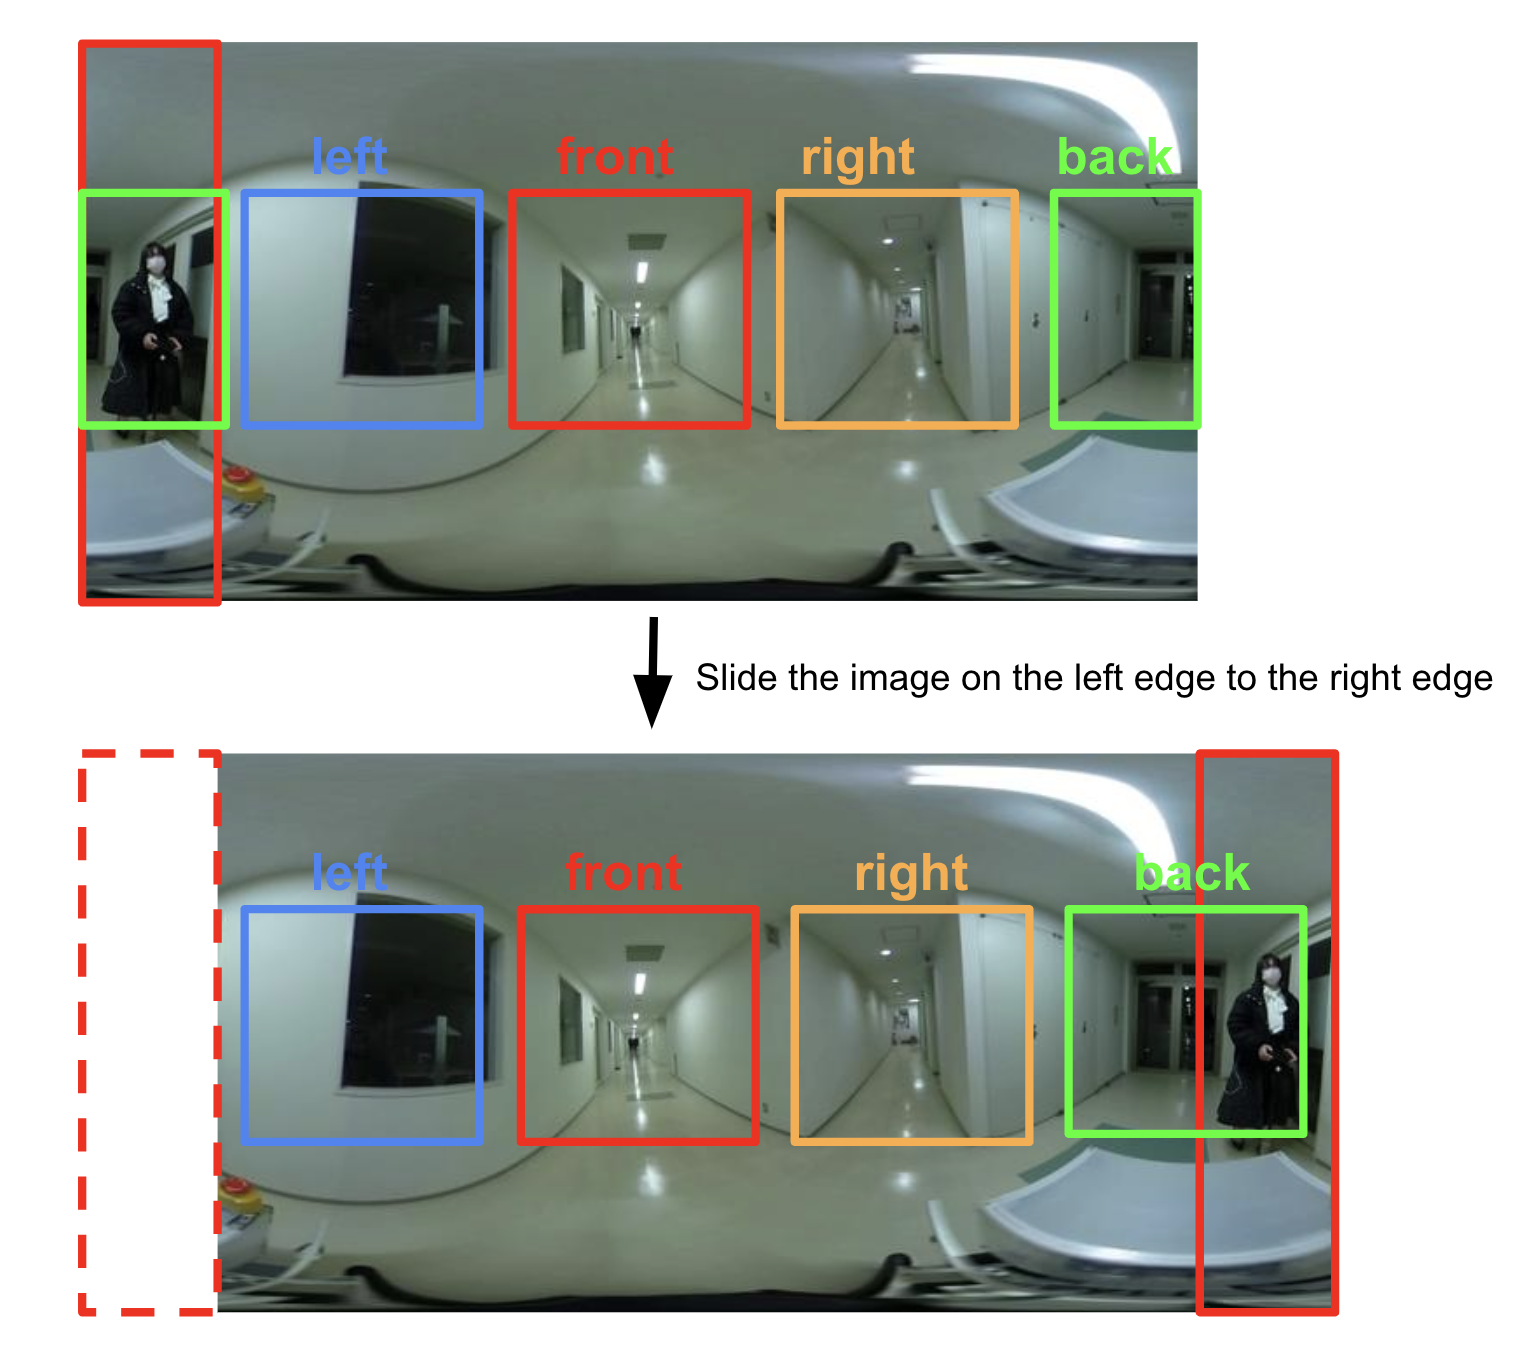
\includegraphics[width=10cm]{../images/image_proc2.png}
        %\caption{Preprocessing of spherical camera images.}
        %\label{figure::image_proc_fig}
        %\end{figure}